\documentclass{article}

\usepackage{graphicx}
\usepackage{tikz}
\usepackage{tikzsymbols}
\usetikzlibrary{calc,patterns,shapes.geometric}
\pagestyle{empty}
\usepackage[margin=0pt]{geometry}
\geometry{papersize={14in,12in}}

\def\centerarc[#1](#2)(#3:#4:#5){\draw[#1] ($(#2)+({#5*cos(#3)},{#5*sin(#3)})$) arc (#3:#4:#5);}

\begin{document}
	\begin{figure}
		\centering
		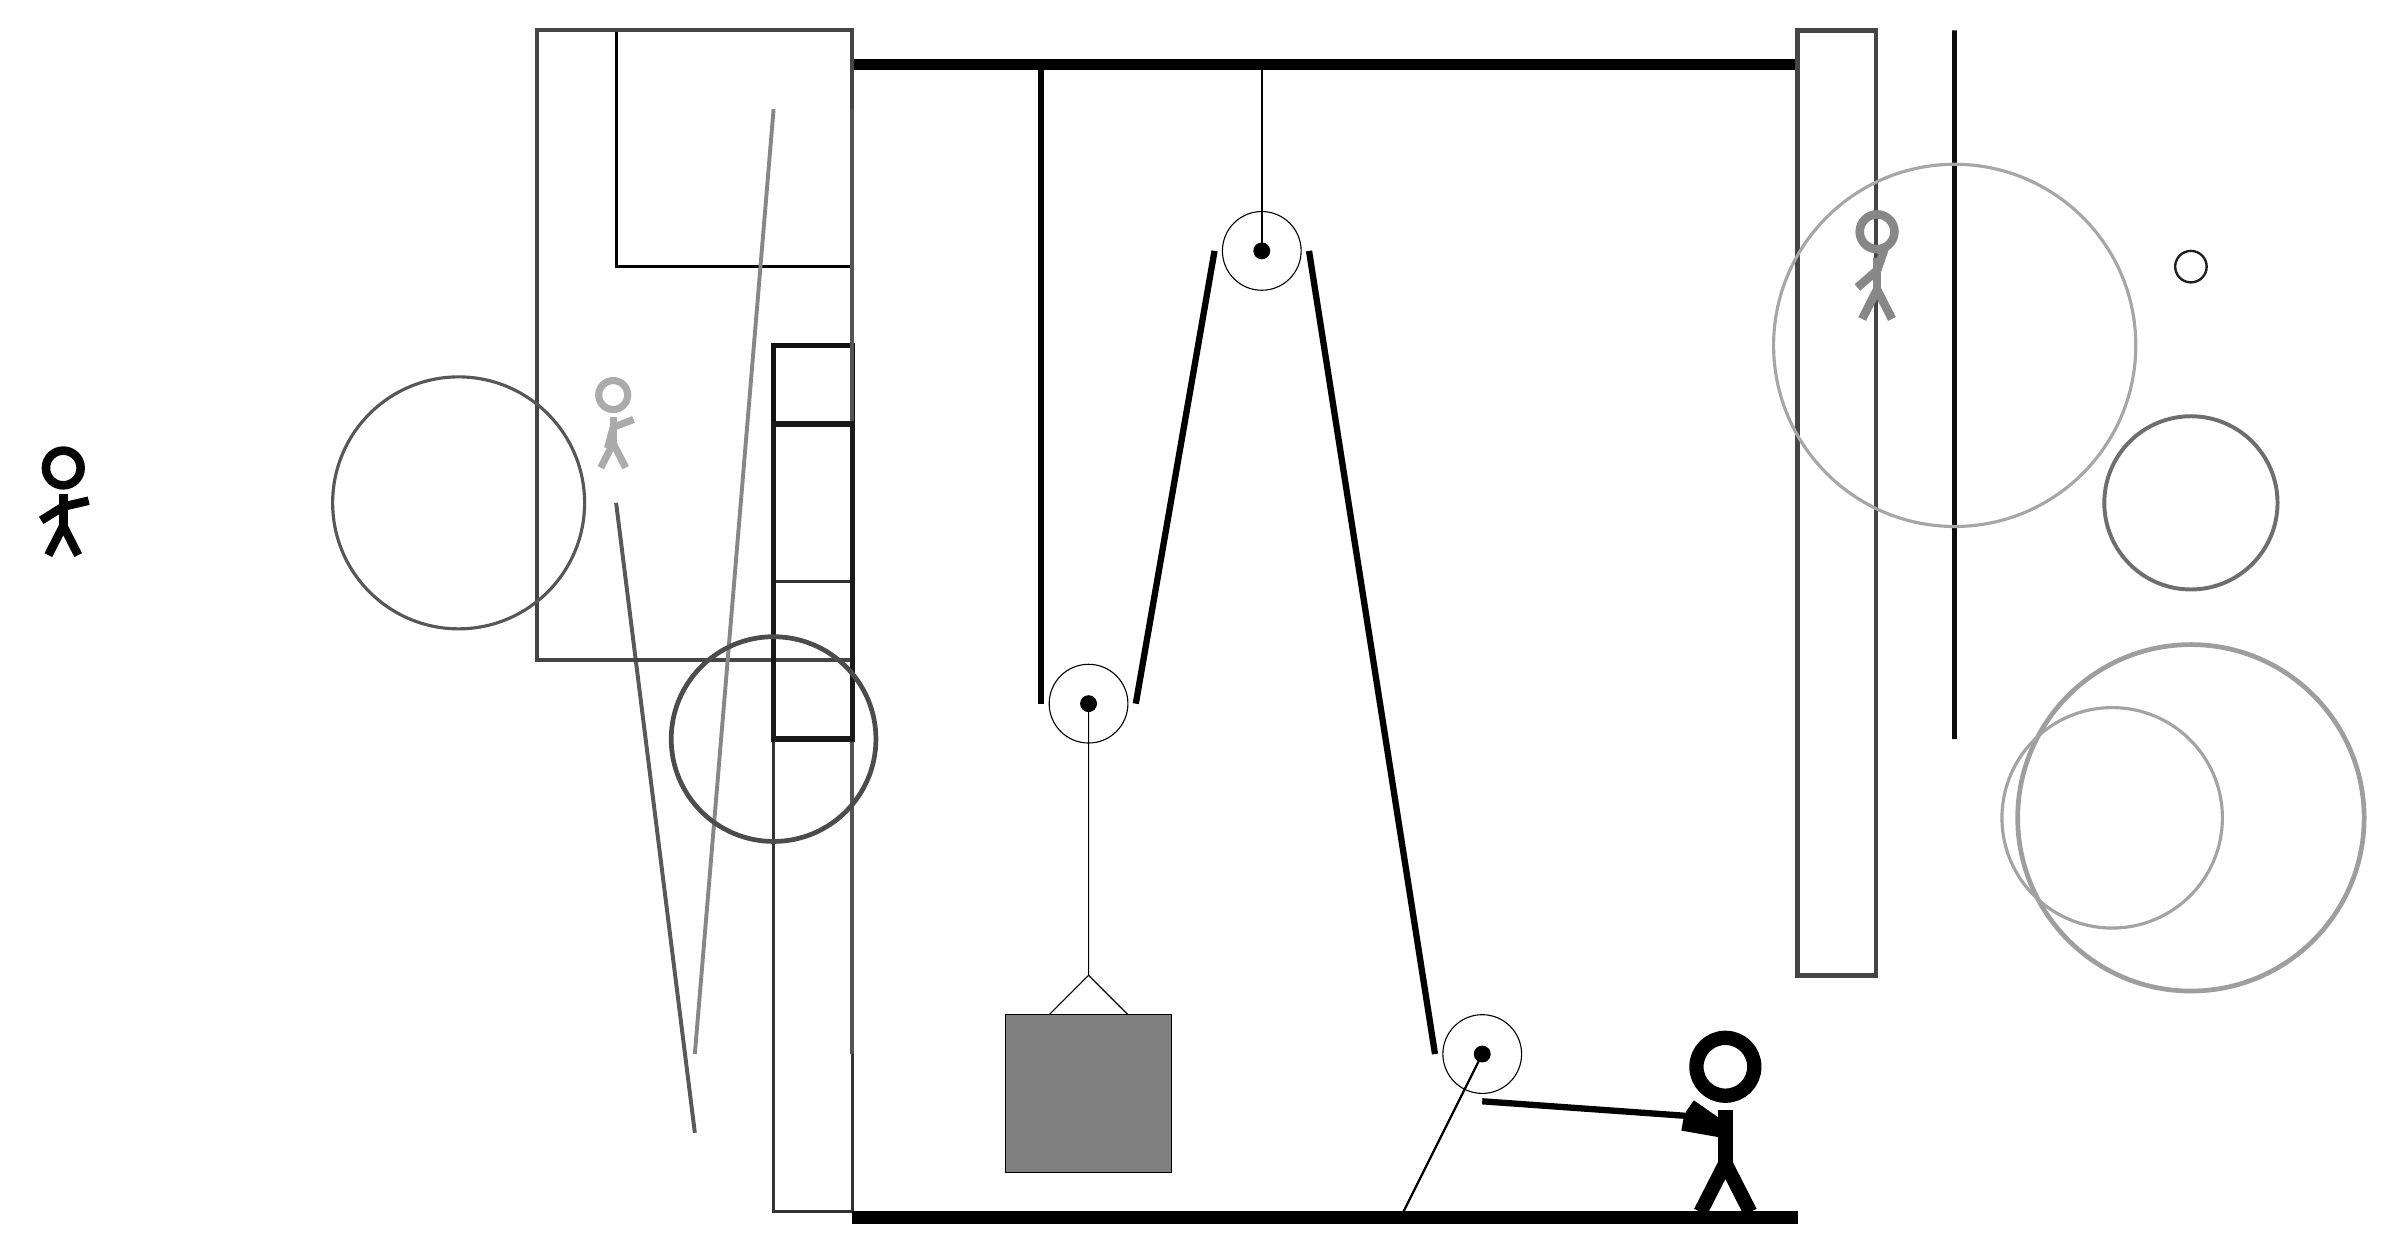
\begin{tikzpicture}
			%%%%% START %%%%%
			
			\draw[fill=black] (-2, 11.5) rectangle (10, 11.625);
			
			\draw (3.2, 9.2) circle (0.5);
			\draw[fill=black] (3.2, 9.2) circle (0.1);
			\draw[thick] (3.2, 9.2) -- (3.2, 11.5);
			
			\draw (6, -1) circle (0.5);
			\draw[fill=black] (6, -1) circle (0.1);
			\draw[thick] (6, -1) -- (5, -3);
			
			\draw (1, 3.45) circle (0.5);
			\draw[fill=black] (1, 3.45) circle (0.1);
			
			\draw (1, 3.45) -- (1, 0.0) -- (0.5, -0.5);
			\draw (1, 0.0) -- (1.5, -0.5);
			\draw[fill=black!50] (-0.05, -0.5) rectangle (2.05, -2.5);
			
			\draw[line width=0.7mm, color=black!95] (12, 3) rectangle (12, 12);
			
			\draw[line width=0.4mm, color=black!35] (10, 2) rectangle (10, 11);
			\draw[line width=0.4mm, color=black!80] (-2, 5) rectangle (-3, -3);
			\draw[line width=0.6mm, color=black!73] (10, 12) rectangle (11, 0);
			\node[line width=0.3mm, color=black!33] at (-5, 7) {\Strichmaxerl[5][75][21]};
			\draw[line width=0.4mm, color=black!100] (-3, 8) rectangle (-3, 3);
			
			\draw[line width=0.5mm, color=black!65](-5, 6) -- (-4, -2);
			
			\draw[line width=0.4mm, color=black!100] (-2, 9) rectangle (-5, 12);
			\draw[line width=0.5mm, color=black!73] (-2, 4) rectangle (-6, 12);
			
			\draw [line width=0.6mm, color=black!38](15, 2) circle (2.2);
			
			\draw [line width=0.4mm, color=black!36](14, 2) circle (1.4);
			\draw [line width=0.3mm, color=black!88](15, 9) circle (0.2);
			\node[line width=0.5mm, color=black!98] at (-12, 6) {\Strichmaxerl[6][32][13]};
			\draw[line width=0.6mm, color=black!93] (-3, 8) rectangle (-2, 3);
			\draw [line width=0.4mm, color=black!35](12, 8) circle (2.3);
			\draw[line width=0.5mm, color=black!47](-3, 11) -- (-4, -1);
			
			\draw[line width=0.5mm, color=black!67] (-2, -1) rectangle (-2, 11);
			\draw [line width=0.4mm, color=black!66](-7, 6) circle (1.6);
			\node[line width=0.6mm, color=black!47] at (11, 9) {\Strichmaxerl[6][41][71]};
			\draw [line width=0.5mm, color=black!57](15, 6) circle (1.1);
			\draw[line width=0.7mm, color=black!90] (-3, 7) rectangle (-2, 3);
			\draw [line width=0.6mm, color=black!70](-3, 3) circle (1.3);
			
			\draw[line width=0.8mm] (0.4, 11.5) -- (0.4, 3.45);
			\centerarc[line width=0.8mm](1, 3.45)(180:360:0.6);
			\draw[line width=0.8mm](1.6, 3.45) -- (2.6, 9.2);
			\centerarc[line width=0.8mm](3.2, 9.2)(0:180:0.6);
			\draw[line width=0.8mm](3.8, 9.2) -- (5.4, -1);
			\centerarc[line width=0.8mm](6, -1)(180:270:0.6);
			\draw[line width=0.8mm](6, -1.6) -- (8.8, -1.8);
			
			\node at (9, -1.9) {\Strichmaxerl[10][-35][170]};
			
			\draw[fill=black] (-2, -3) rectangle (10, -3.15);
			
			%%%%% END %%%%%
		\end{tikzpicture}
	\end{figure}	
\end{document}